% compile with: pdflatex -shell-escape filename.tex
\documentclass[crop,tikz,convert=pdf2svg]{standalone}
\usepackage{tikz}
\usetikzlibrary{backgrounds}
\usetikzlibrary{calc}
\usetikzlibrary{decorations.pathreplacing}
\usetikzlibrary{matrix}
\usetikzlibrary{positioning}

\tikzset{
  label/.style={
    anchor=west,
    minimum width=60pt,
    text width=60pt,
  },
}

\tikzset{
  ncbar angle/.initial=90,
  ncbar/.style={
    to path=(\tikztostart)
    -- ($(\tikztostart)!#1!\pgfkeysvalueof{/tikz/ncbar angle}:(\tikztotarget)$)
    -- ($(\tikztotarget)!($(\tikztostart)!#1!\pgfkeysvalueof{/tikz/ncbar angle}:(\tikztotarget)$)!\pgfkeysvalueof{/tikz/ncbar angle}:(\tikztostart)$)
    -- (\tikztotarget)
  },
  ncbar/.default=0.5cm,
}

\tikzset{
  bracket/.style={ncbar=-0.25cm}
}

\begin{document}

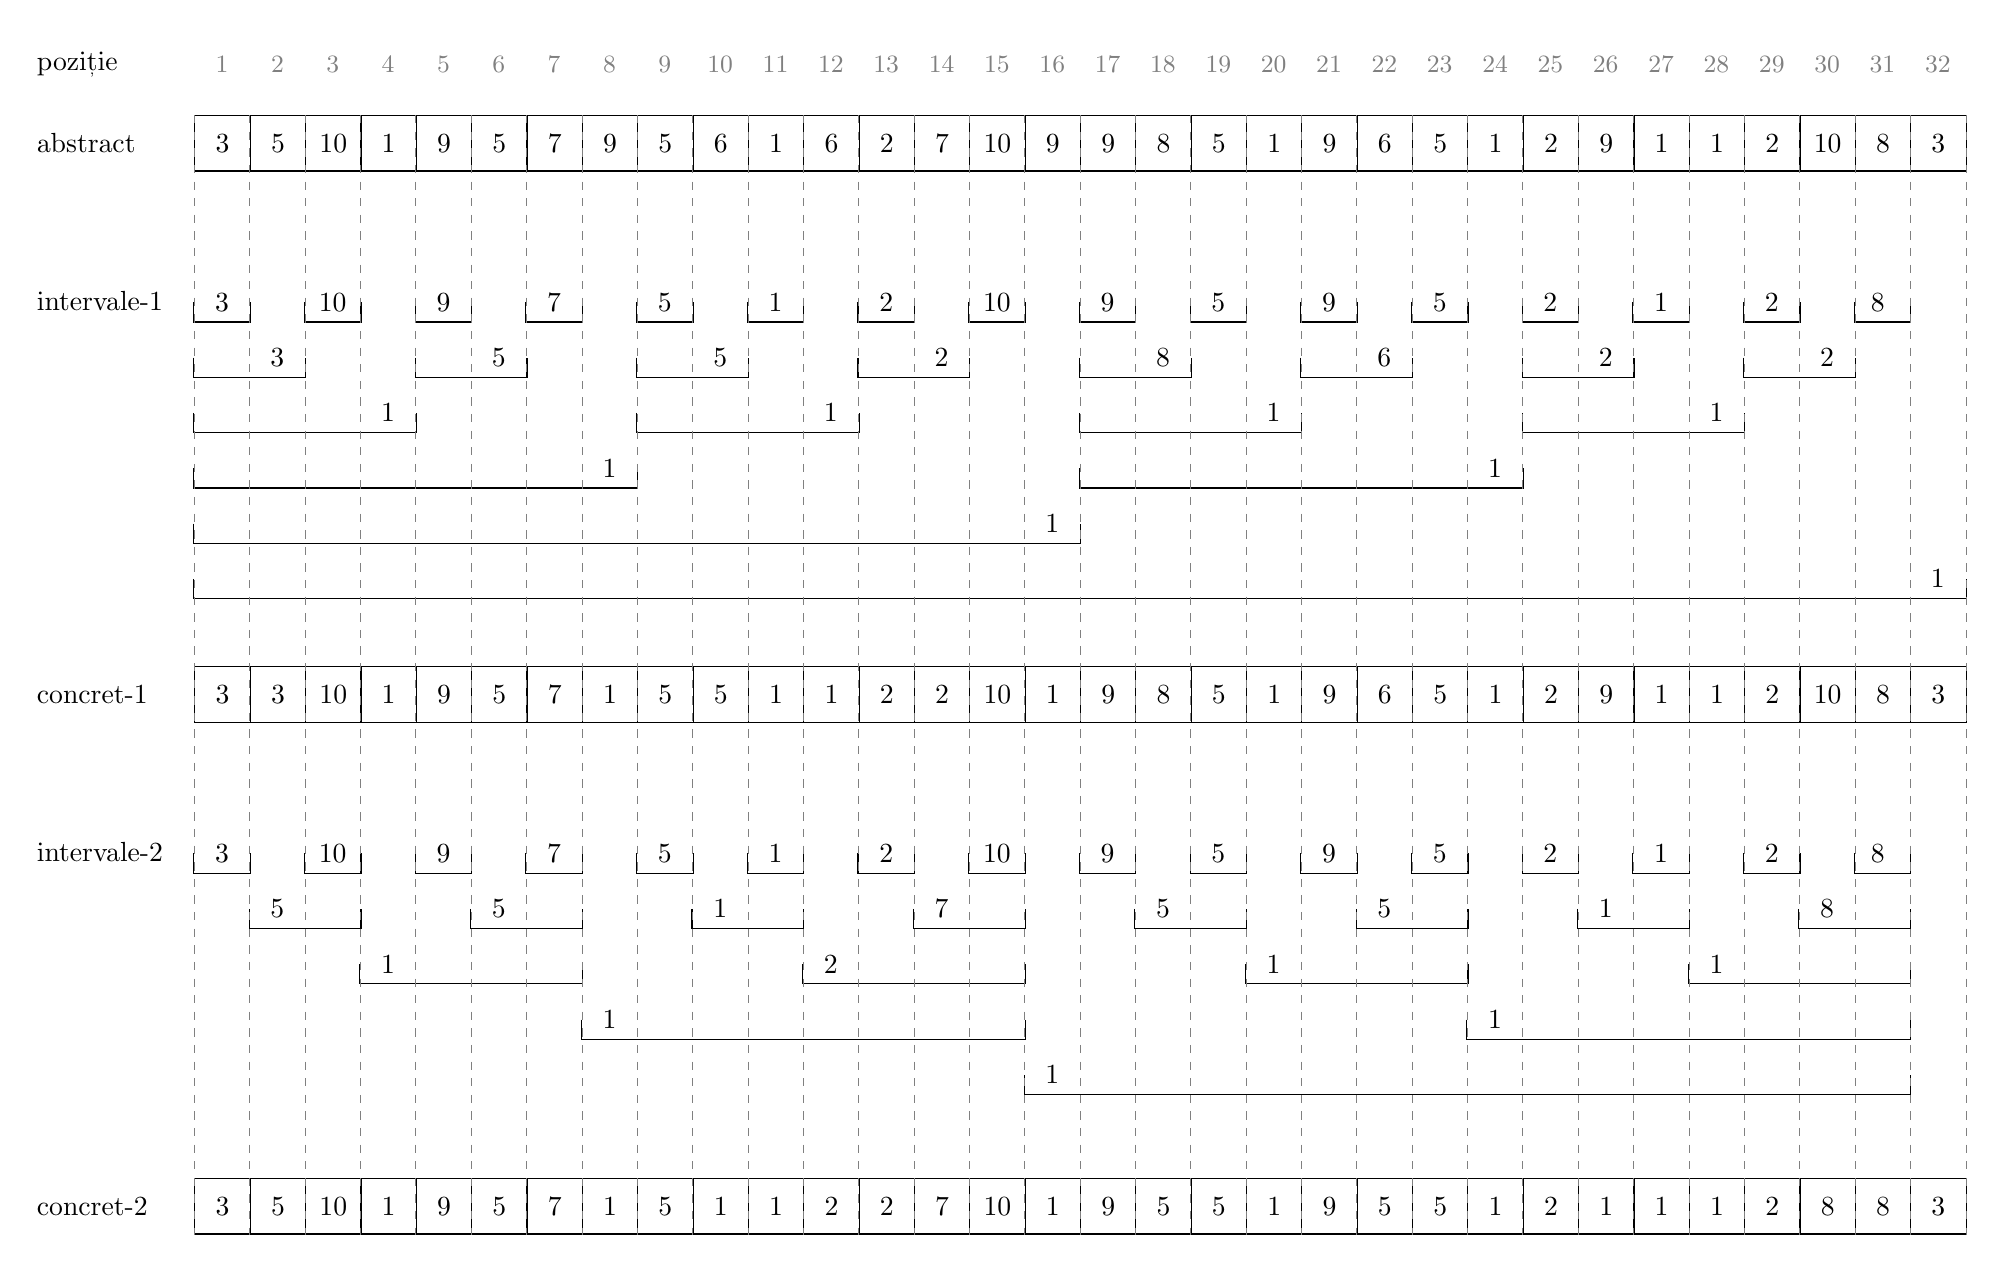
\begin{tikzpicture}
  % First row: indices
  \node[label] at (0, 0) {poziție};

  \matrix[right] (index) at (2, 0) [
    matrix of nodes,
    nodes={anchor=center, minimum size=20pt, color=black!50, font=\small},
  ] {
    1 & 2 & 3 & 4 & 5 & 6 & 7 & 8 & 9 & 10 & 11 & 12 & 13 & 14 & 15 & 16 & 17 & 18 & 19 & 20 & 21 & 22 & 23 & 24 & 25 & 26 & 27 & 28 & 29 & 30 & 31 & 32\\
  };

  % Second row: abstract values
  \node[label] at (0, -1) {abstract};

  \matrix[right] (abstract) at (2, -1) [
    matrix of nodes,
    nodes={draw, anchor=center, minimum size=20pt},
    column sep=-\pgflinewidth,
    row sep=-\pgflinewidth
  ] {
    3 & 5 & 10 & 1 & 9 & 5 & 7 & 9 & 5 & 6 & 1 & 6 & 2 & 7 & 10 & 9 & 9 & 8 & 5 & 1 & 9 & 6 & 5 & 1 & 2 & 9 & 1 & 1 & 2 & 10 & 8 & 3\\
  };

  % Third row: partial min intervals (left)
  \node[label] at (0, -3) {intervale-1};

  \matrix[below right=-13pt and 0pt] (intl) at (2, -3) [
    matrix of nodes,
    nodes={anchor=center, minimum size=20pt},
  ] {
    3 & \  & 10 & \  & 9 & \  & 7 & \  & 5 & \  & 1 & \  & 2 & \  & 10 & \  & 9 & \  & 5 & \  & 9 & \ & 5  & \  & 2  & \  & 1 & \  & 2  & \  & 8 \ \\
    \  & 3 & \  & \  & \  & 5 & \  & \  & \  & 5 & \  & \  & \  & 2 & \  & \  & \  & 8 & \  & \  & \  & 6 & \  & \  & \  & 2 & \  & \  & \  & 2 & \  & \ \\
    \  & \  & \  & 1 & \  & \  & \  & \  & \  & \  & \  & 1 & \  & \  & \  & \  & \  & \  & \  & 1 & \  & \  & \  & \  & \  & \  & \  & 1  & \  & \  & \  & \ \\
    \  & \  & \  & \  & \  & \  & \  & 1 & \  & \  & \  & \  & \  & \  & \  & \  & \  & \  & \  & \  & \  & \  & \  & 1 & \  & \  & \  & \  & \  & \  & \  & \ \\
    \  & \  & \  & \  & \  & \  & \  & \  & \  & \  & \  & \  & \  & \  & \  & 1 & \  & \  & \  & \  & \  & \  & \  & \  & \  & \  & \  & \  & \  & \  & \ & \ \\
    \  & \  & \  & \  & \  & \  & \  & \  & \  & \  & \  & \  & \  & \  & \  & \  & \  & \  & \  & \  & \  & \  & \  & \  & \  & \  & \  & \  & \  & \  & \ & 1\\
  };

  \foreach \x in {1,3,...,31} {
    \draw (intl-1-\x.west) to [bracket] (intl-1-\x.east);
  }
  \draw (intl-2-1.west) to [bracket] (intl-2-2.east);
  \draw (intl-2-5.west) to [bracket] (intl-2-6.east);
  \draw (intl-2-9.west) to [bracket] (intl-2-10.east);
  \draw (intl-2-13.west) to [bracket] (intl-2-14.east);
  \draw (intl-2-17.west) to [bracket] (intl-2-18.east);
  \draw (intl-2-21.west) to [bracket] (intl-2-22.east);
  \draw (intl-2-25.west) to [bracket] (intl-2-26.east);
  \draw (intl-2-29.west) to [bracket] (intl-2-30.east);

  \draw (intl-3-1.west) to [bracket] (intl-3-4.east);
  \draw (intl-3-9.west) to [bracket] (intl-3-12.east);
  \draw (intl-3-17.west) to [bracket] (intl-3-20.east);
  \draw (intl-3-25.west) to [bracket] (intl-3-28.east);

  \draw (intl-4-1.west) to [bracket] (intl-4-8.east);
  \draw (intl-4-17.west) to [bracket] (intl-4-24.east);

  \draw (intl-5-1.west) to [bracket] (intl-5-16.east);

  \draw (intl-6-1.west) to [bracket] (intl-6-32.east);

  % Fourth row: concrete values (left)
  \node[label] at (0, -8) {concret-1};

  \matrix[right] (concrete1) at (2, -8) [
    matrix of nodes,
    nodes={draw, anchor=center, minimum size=20pt},
    column sep=-\pgflinewidth,
    row sep=-\pgflinewidth
  ] {
    3 & 3 & 10 & 1 & 9 & 5 & 7 & 1 & 5 & 5 & 1 & 1 & 2 & 2 & 10 & 1 & 9 & 8 & 5 & 1 & 9 & 6 & 5 & 1 & 2 & 9 & 1 & 1 & 2 & 10 & 8 & 3\\
  };

  % Fifth row: partial min intervals (right)
  \node[label] at (0, -10) {intervale-2};

  \matrix[below right=-13pt and 0pt] (intr) at (2, -10) [
    matrix of nodes,
    nodes={anchor=center, minimum size=20pt},
  ] {
    3 & \  & 10 & \  & 9 & \  & 7 & \  & 5 & \  & 1 & \  & 2 & \  & 10 & \  & 9 & \  & 5 & \  & 9 & \ & 5  & \  & 2  & \  & 1 & \  & 2  & \  & 8 \ \\
    \  & 5 & \  & \  & \  & 5 & \  & \  & \  & 1 & \  & \  & \  & 7 & \  & \  & \  & 5 & \  & \  & \  & 5 & \  & \  & \  & 1 & \  & \  & \  & 8 & \  & \ \\
    \  & \  & \  & 1 & \  & \  & \  & \  & \  & \  & \  & 2 & \  & \  & \  & \  & \  & \  & \  & 1 & \  & \  & \  & \  & \  & \  & \  & 1  & \  & \  & \  & \ \\
    \  & \  & \  & \  & \  & \  & \  & 1 & \  & \  & \  & \  & \  & \  & \  & \  & \  & \  & \  & \  & \  & \  & \  & 1 & \  & \  & \  & \  & \  & \  & \  & \ \\
    \  & \  & \  & \  & \  & \  & \  & \  & \  & \  & \  & \  & \  & \  & \  & 1 & \  & \  & \  & \  & \  & \  & \  & \  & \  & \  & \  & \  & \  & \  & \ & \ \\
  };

  \foreach \x in {1,3,...,31} {
    \draw (intr-1-\x.west) to [bracket] (intr-1-\x.east);
  }
  \draw (intr-2-2.west) to [bracket] (intr-2-3.east);
  \draw (intr-2-6.west) to [bracket] (intr-2-7.east);
  \draw (intr-2-10.west) to [bracket] (intr-2-11.east);
  \draw (intr-2-14.west) to [bracket] (intr-2-15.east);
  \draw (intr-2-18.west) to [bracket] (intr-2-19.east);
  \draw (intr-2-22.west) to [bracket] (intr-2-23.east);
  \draw (intr-2-26.west) to [bracket] (intr-2-27.east);
  \draw (intr-2-30.west) to [bracket] (intr-2-31.east);

  \draw (intr-3-4.west) to [bracket] (intr-3-7.east);
  \draw (intr-3-12.west) to [bracket] (intr-3-15.east);
  \draw (intr-3-20.west) to [bracket] (intr-3-23.east);
  \draw (intr-3-28.west) to [bracket] (intr-3-31.east);

  \draw (intr-4-8.west) to [bracket] (intr-4-15.east);
  \draw (intr-4-24.west) to [bracket] (intr-4-31.east);

  \draw (intr-5-16.west) to [bracket] (intr-5-31.east);

  % Sixth row: concrete values (right)
  \node[label] at (0, -14.5) {concret-2};

  \matrix[right] (concrete2) at (2, -14.5) [
    matrix of nodes,
    nodes={draw, anchor=center, minimum size=20pt},
    column sep=-\pgflinewidth,
    row sep=-\pgflinewidth
  ] {
    3 & 5 & 10 & 1 & 9 & 5 & 7 & 1 & 5 & 1 & 1 & 2 & 2 & 7 & 10 & 1 & 9 & 5 & 5 & 1 & 9 & 5 & 5 & 1 & 2 & 1 & 1 & 1 & 2 & 8 & 8 & 3\\
  };

  % Vertical grid lines
  \foreach \x in {1,...,32} {
    \draw [help lines, dashed] (abstract-1-\x.north west) -- (concrete2-1-\x.south west);
  }
  \draw [help lines, dashed] (abstract-1-32.north east) -- (concrete2-1-32.south east);
\end{tikzpicture}

\end{document}
